%%%%%%%%%%%%%%%%%%%%%%%%%%%%%%%%%%%%%%%%%%%%%%%%%%%%%%%%%%%%%%%%%%%%%%
%
% pdflatex  atlas_S.tex 
%
%%%%%%%%%%%%%%%%%%%%%%%%%%%%%%%%%%%%%%%%%%%%%%%%%%%%%%%%%%%%%%%%%%%%%%
%
\documentclass[10pt,landscape,oneside]{article}
\usepackage[top=2cm,left=1cm,right=1cm,bottom=0cm,a3paper]{geometry}

\usepackage{times,latexsym,amssymb}
\usepackage{eulervm} % math font
\pagestyle{empty}

\usepackage{amssymb} 
\usepackage{nicefrac} 
\usepackage{pagecolor}
\usepackage{natbib}
%
\usepackage{xcolor,graphicx,transparent}


%\pagecolor{black}
\pagecolor{white}
%%%%%%%%%%%%%%%%%%%%%%%%%%%%%%%%%%%%%%%%%%%%%%%%%%%%%%%%%%%%%%%%%%%%%%
\begin{document}

\begin{center}
\noindent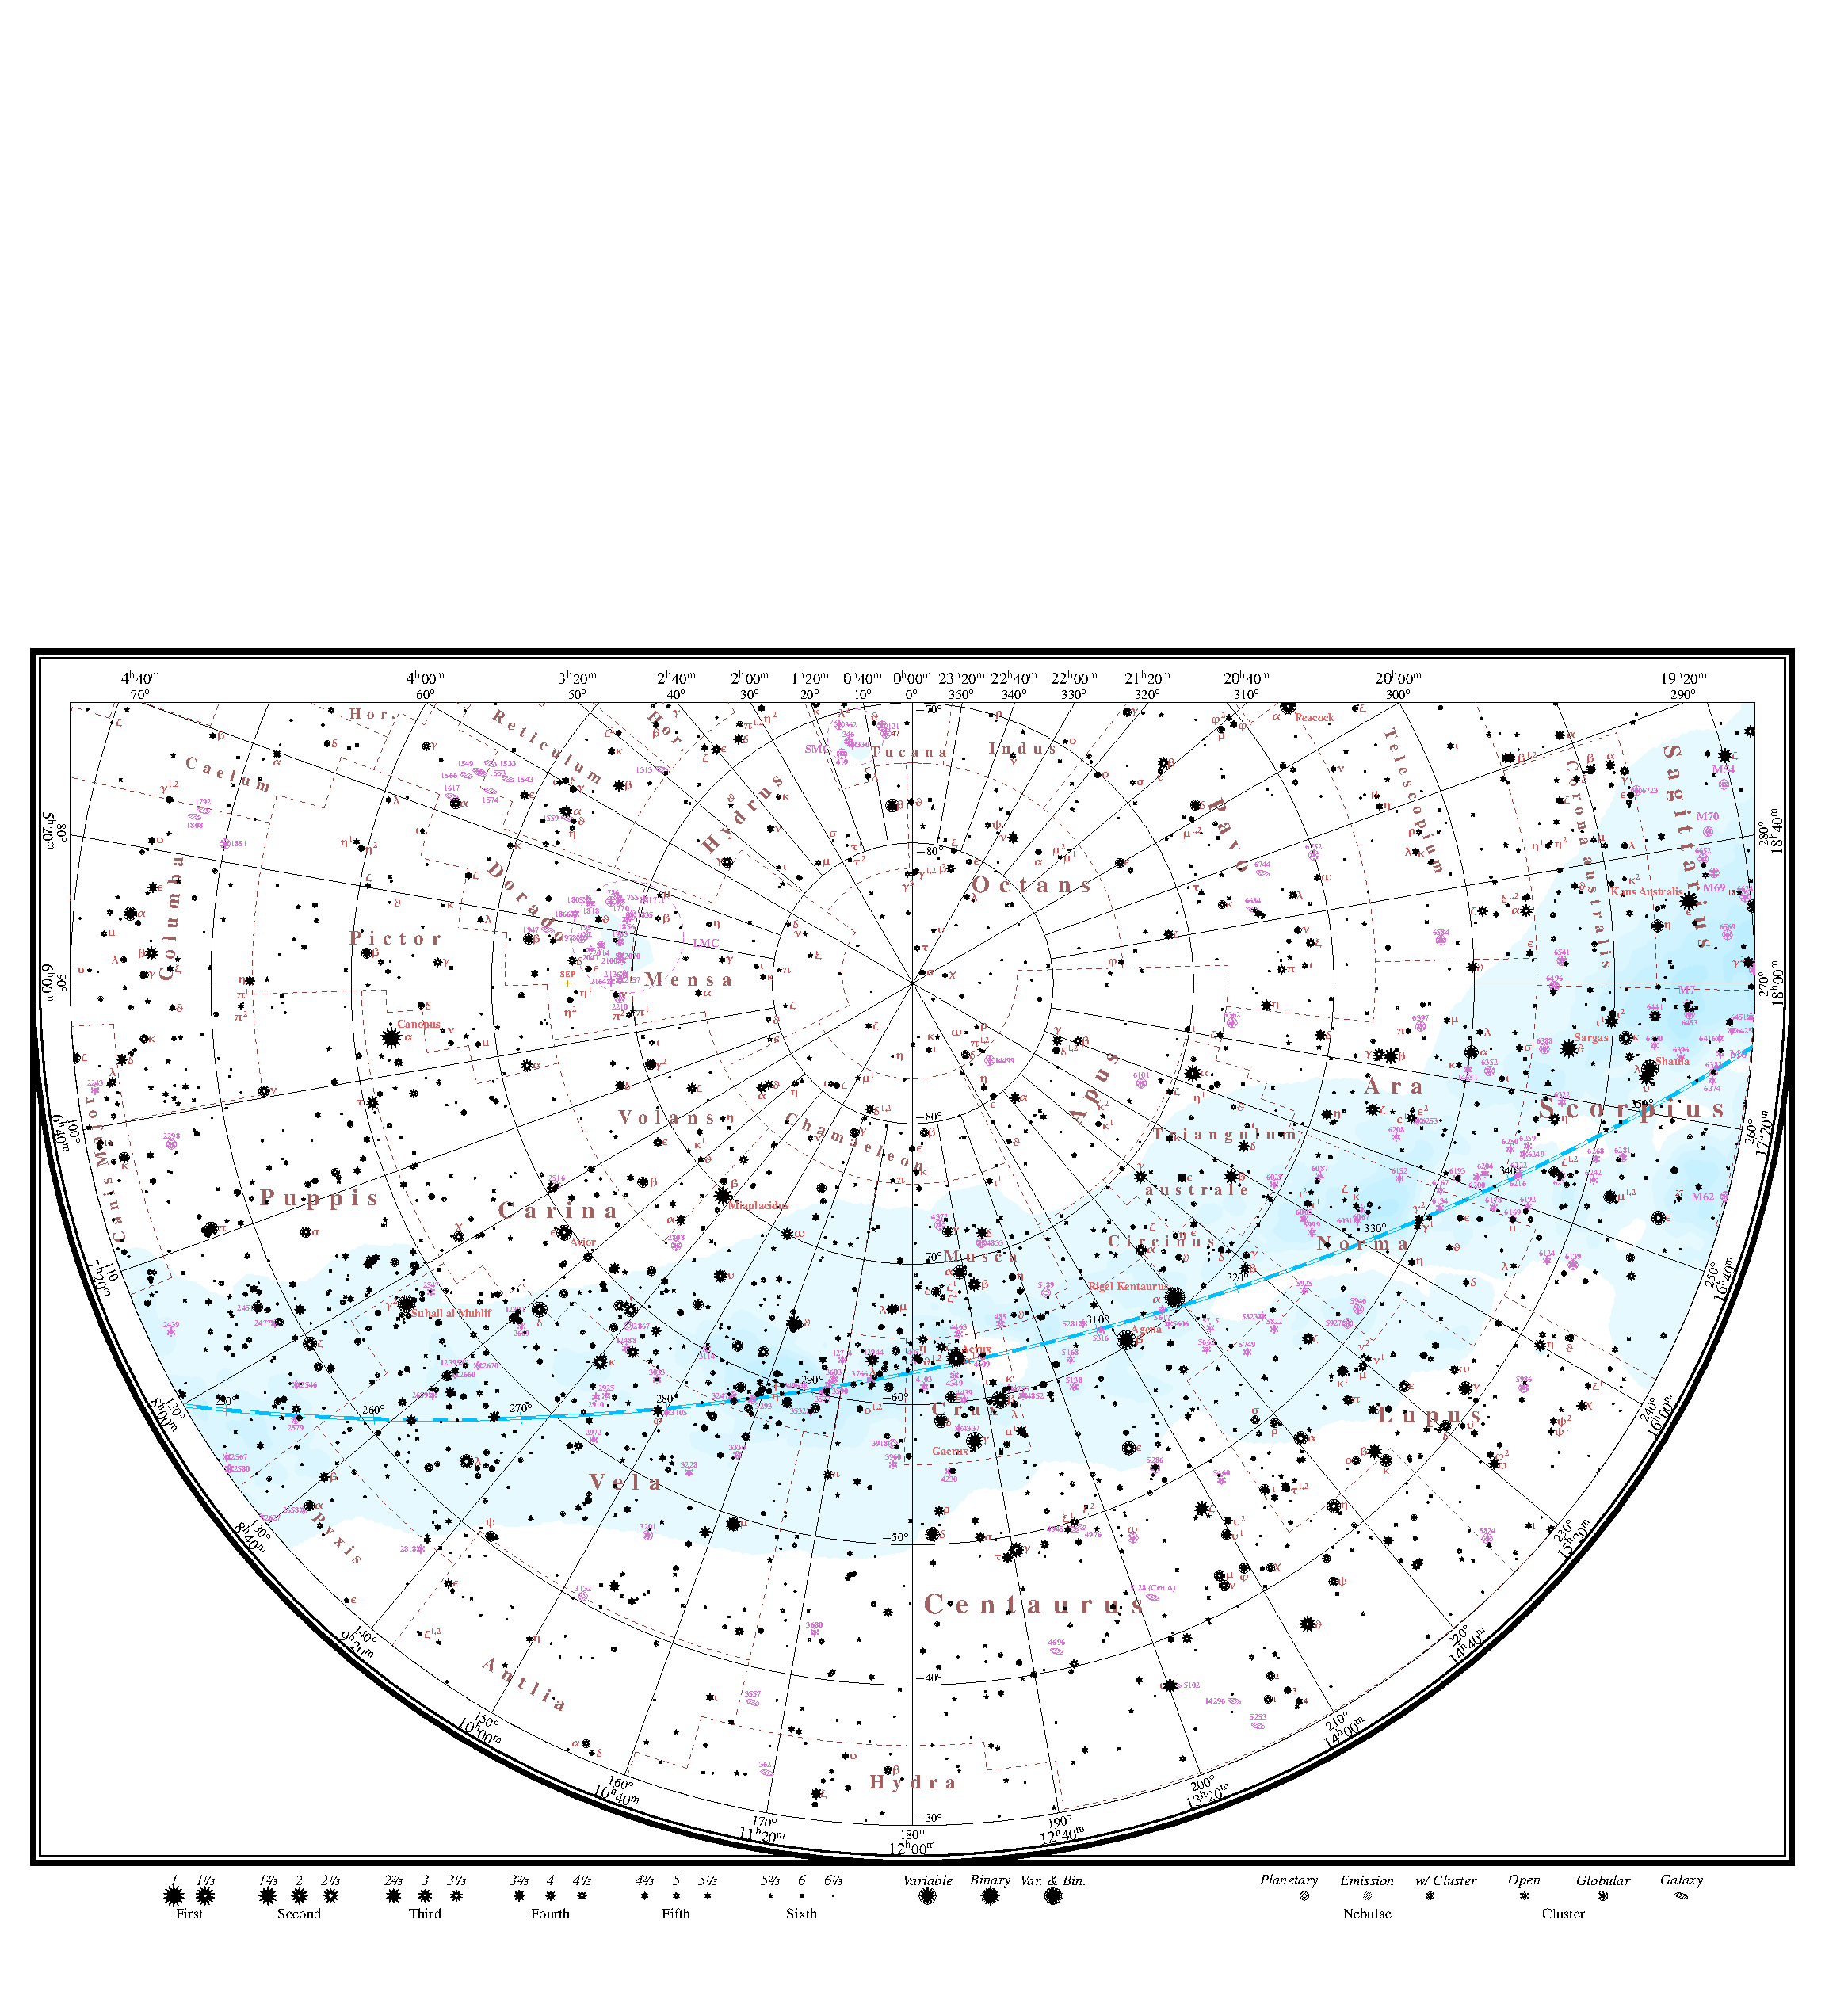
\includegraphics[height=\textheight,trim= 0.0cm -0.5cm 0.0cm 13.85cm,clip]{TabulaVIII.pdf}\\[-1.025\textheight]\hfill\large~Tabula I-S\hspace{25mm}
\clearpage
%
\noindent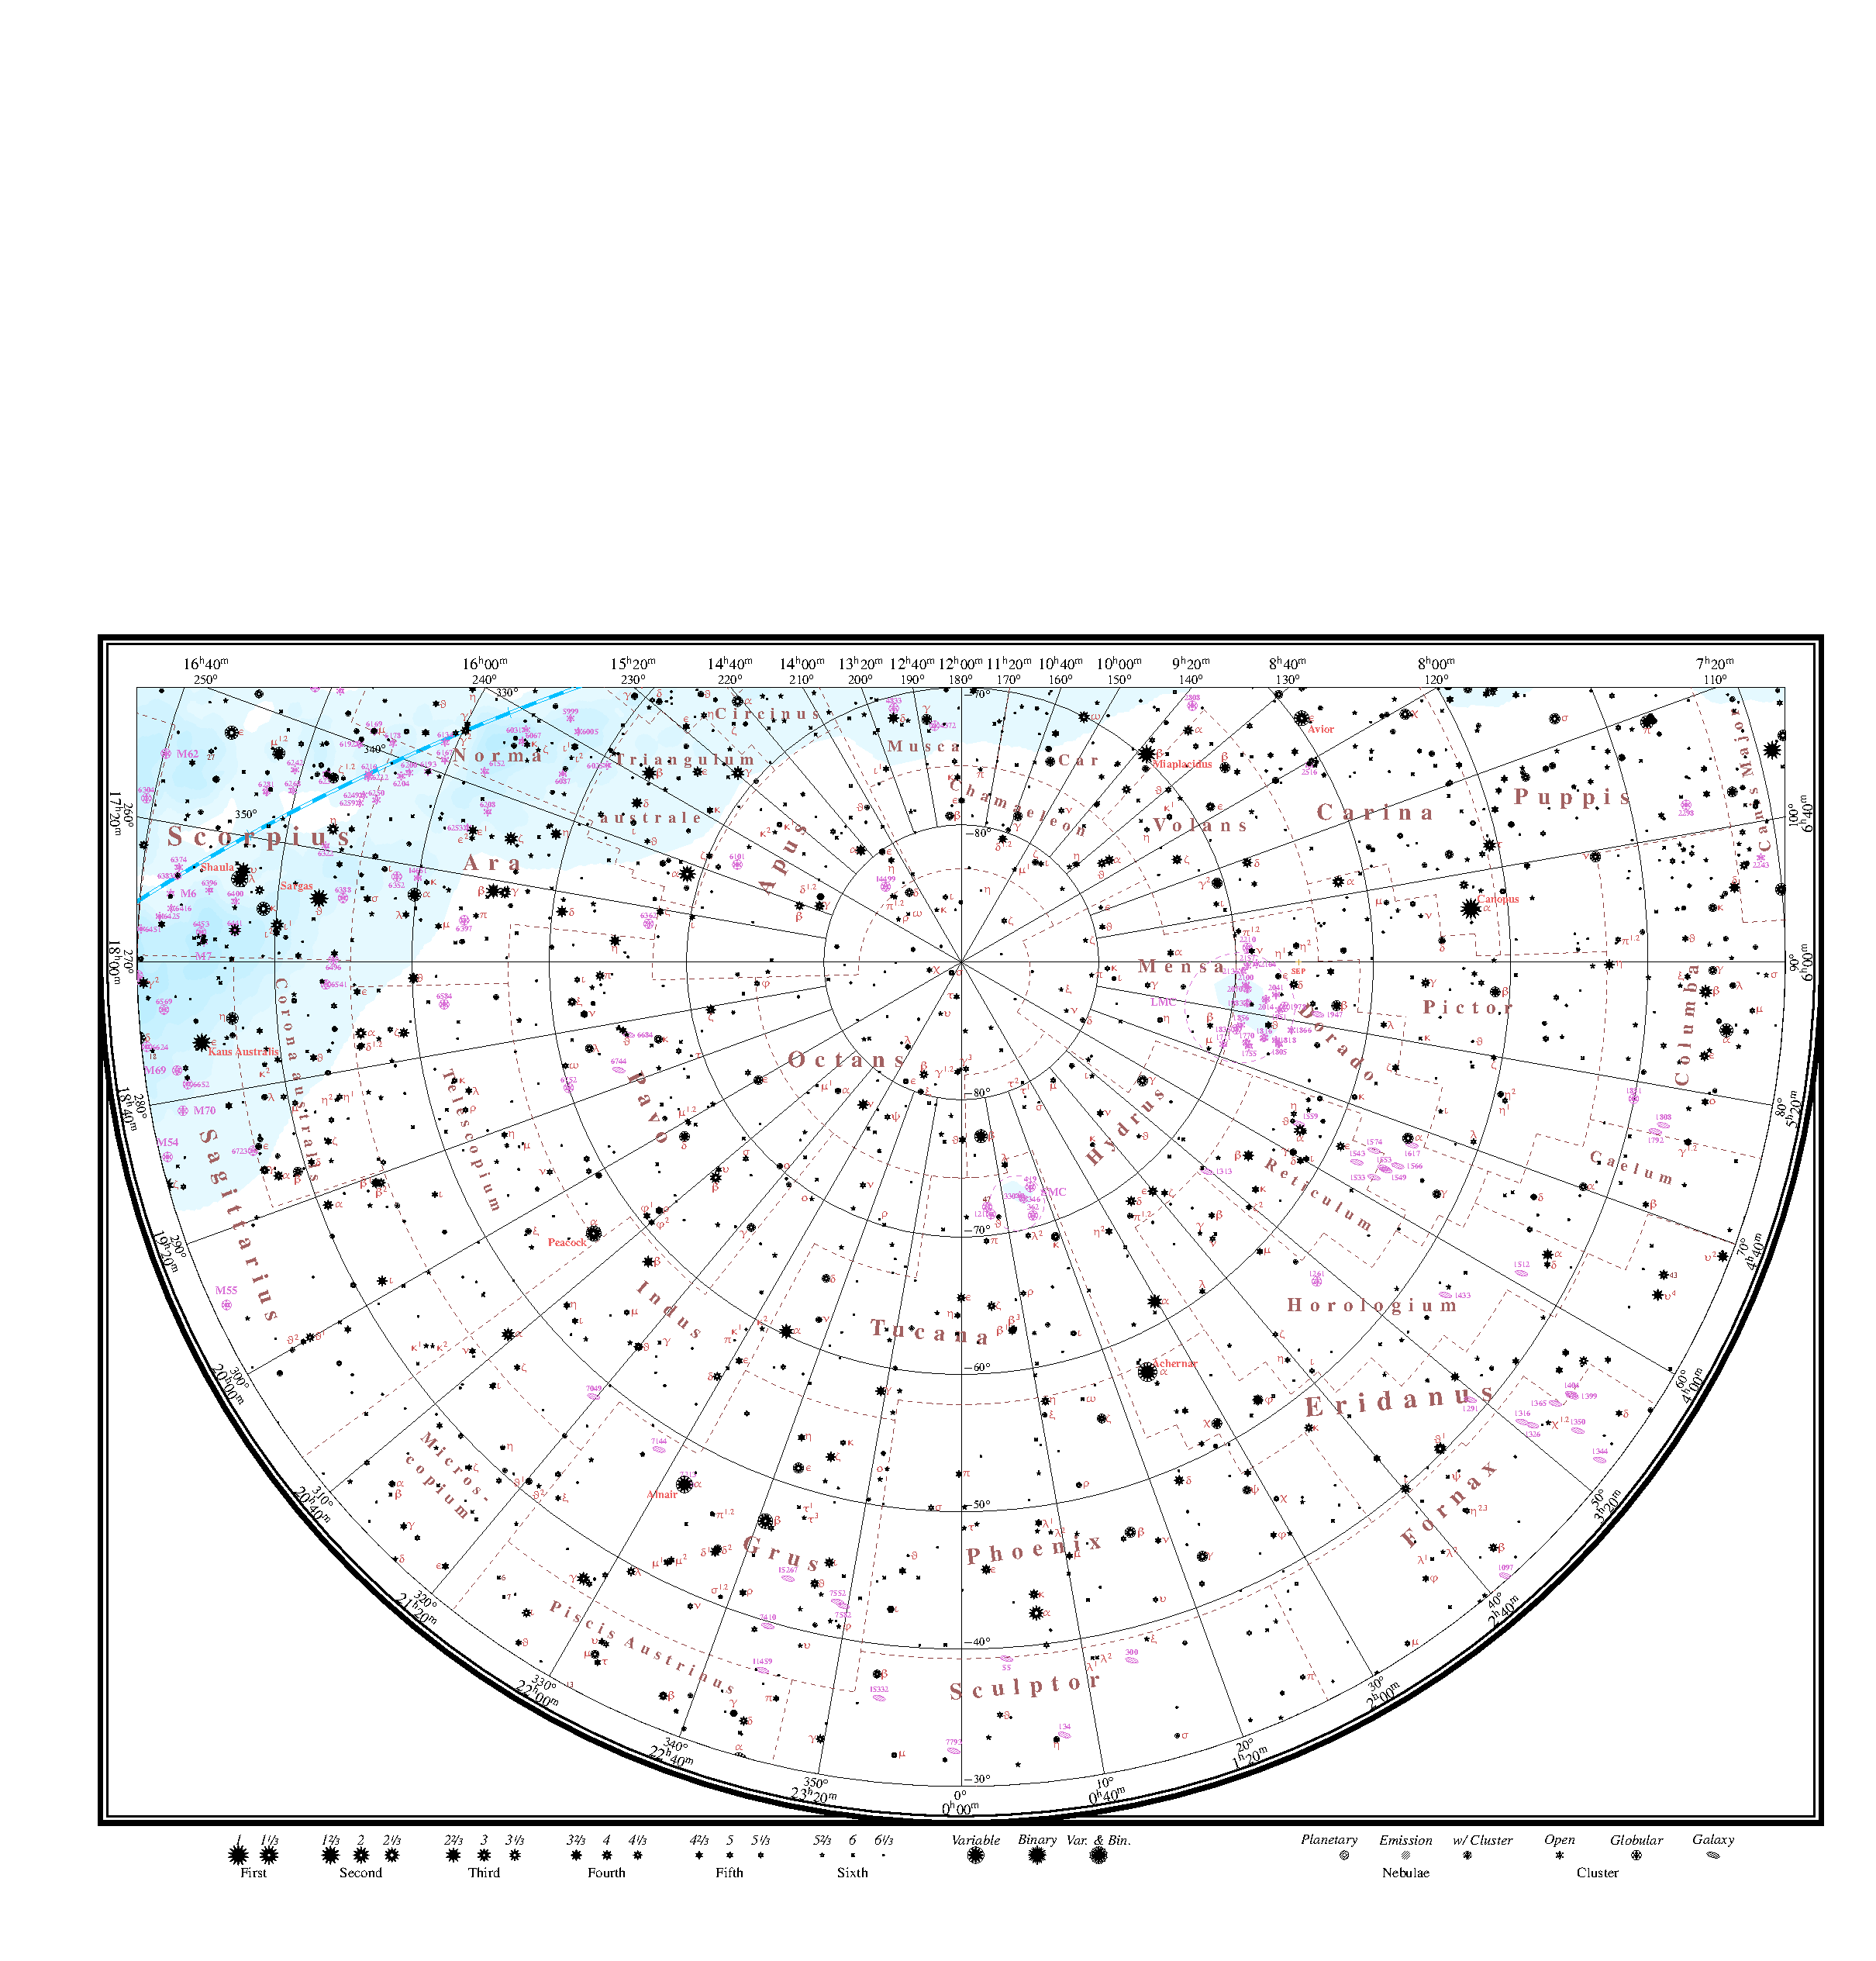
\includegraphics[height=\textheight,trim= 0.0cm -0.5cm 0.0cm 13.85cm,clip]{TabulaVII.pdf}\\[-1.025\textheight]\hfill\large~Tabula II-S\hspace{18mm}
\clearpage
%
\noindent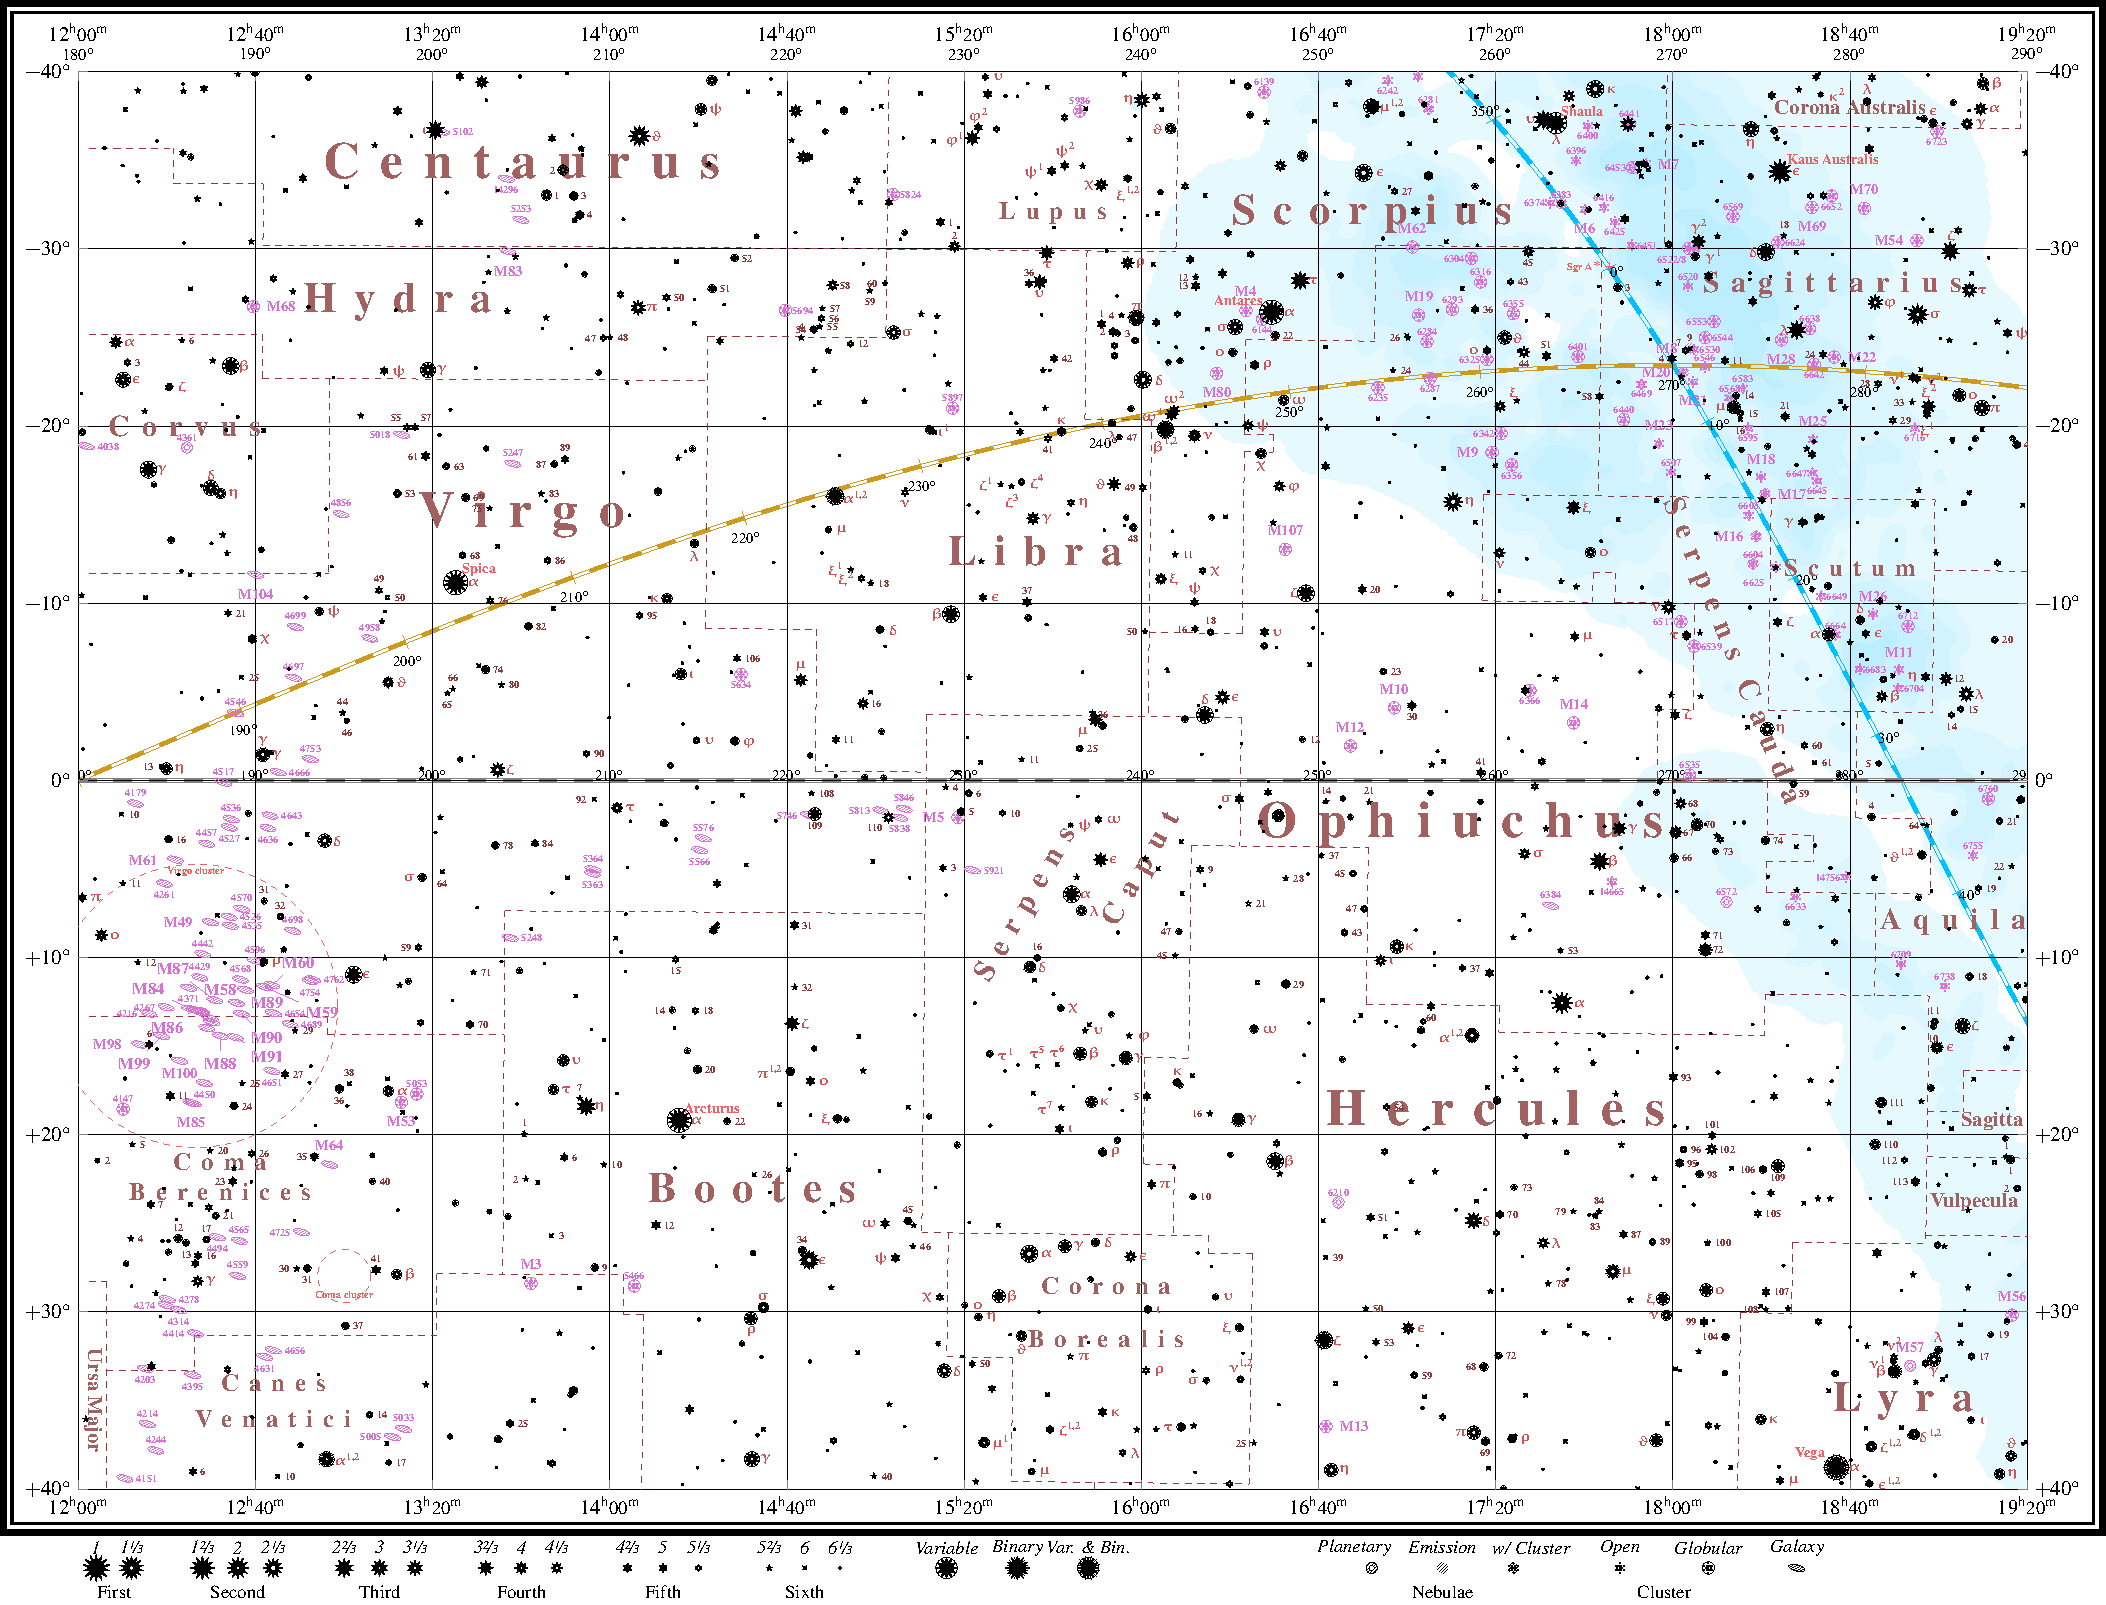
\includegraphics[height=0.963\textheight]{TabulaV_S.pdf}\\[-0.985\textheight]\hfill\large~Tabula III-S\hspace{25mm}
\clearpage
%
\noindent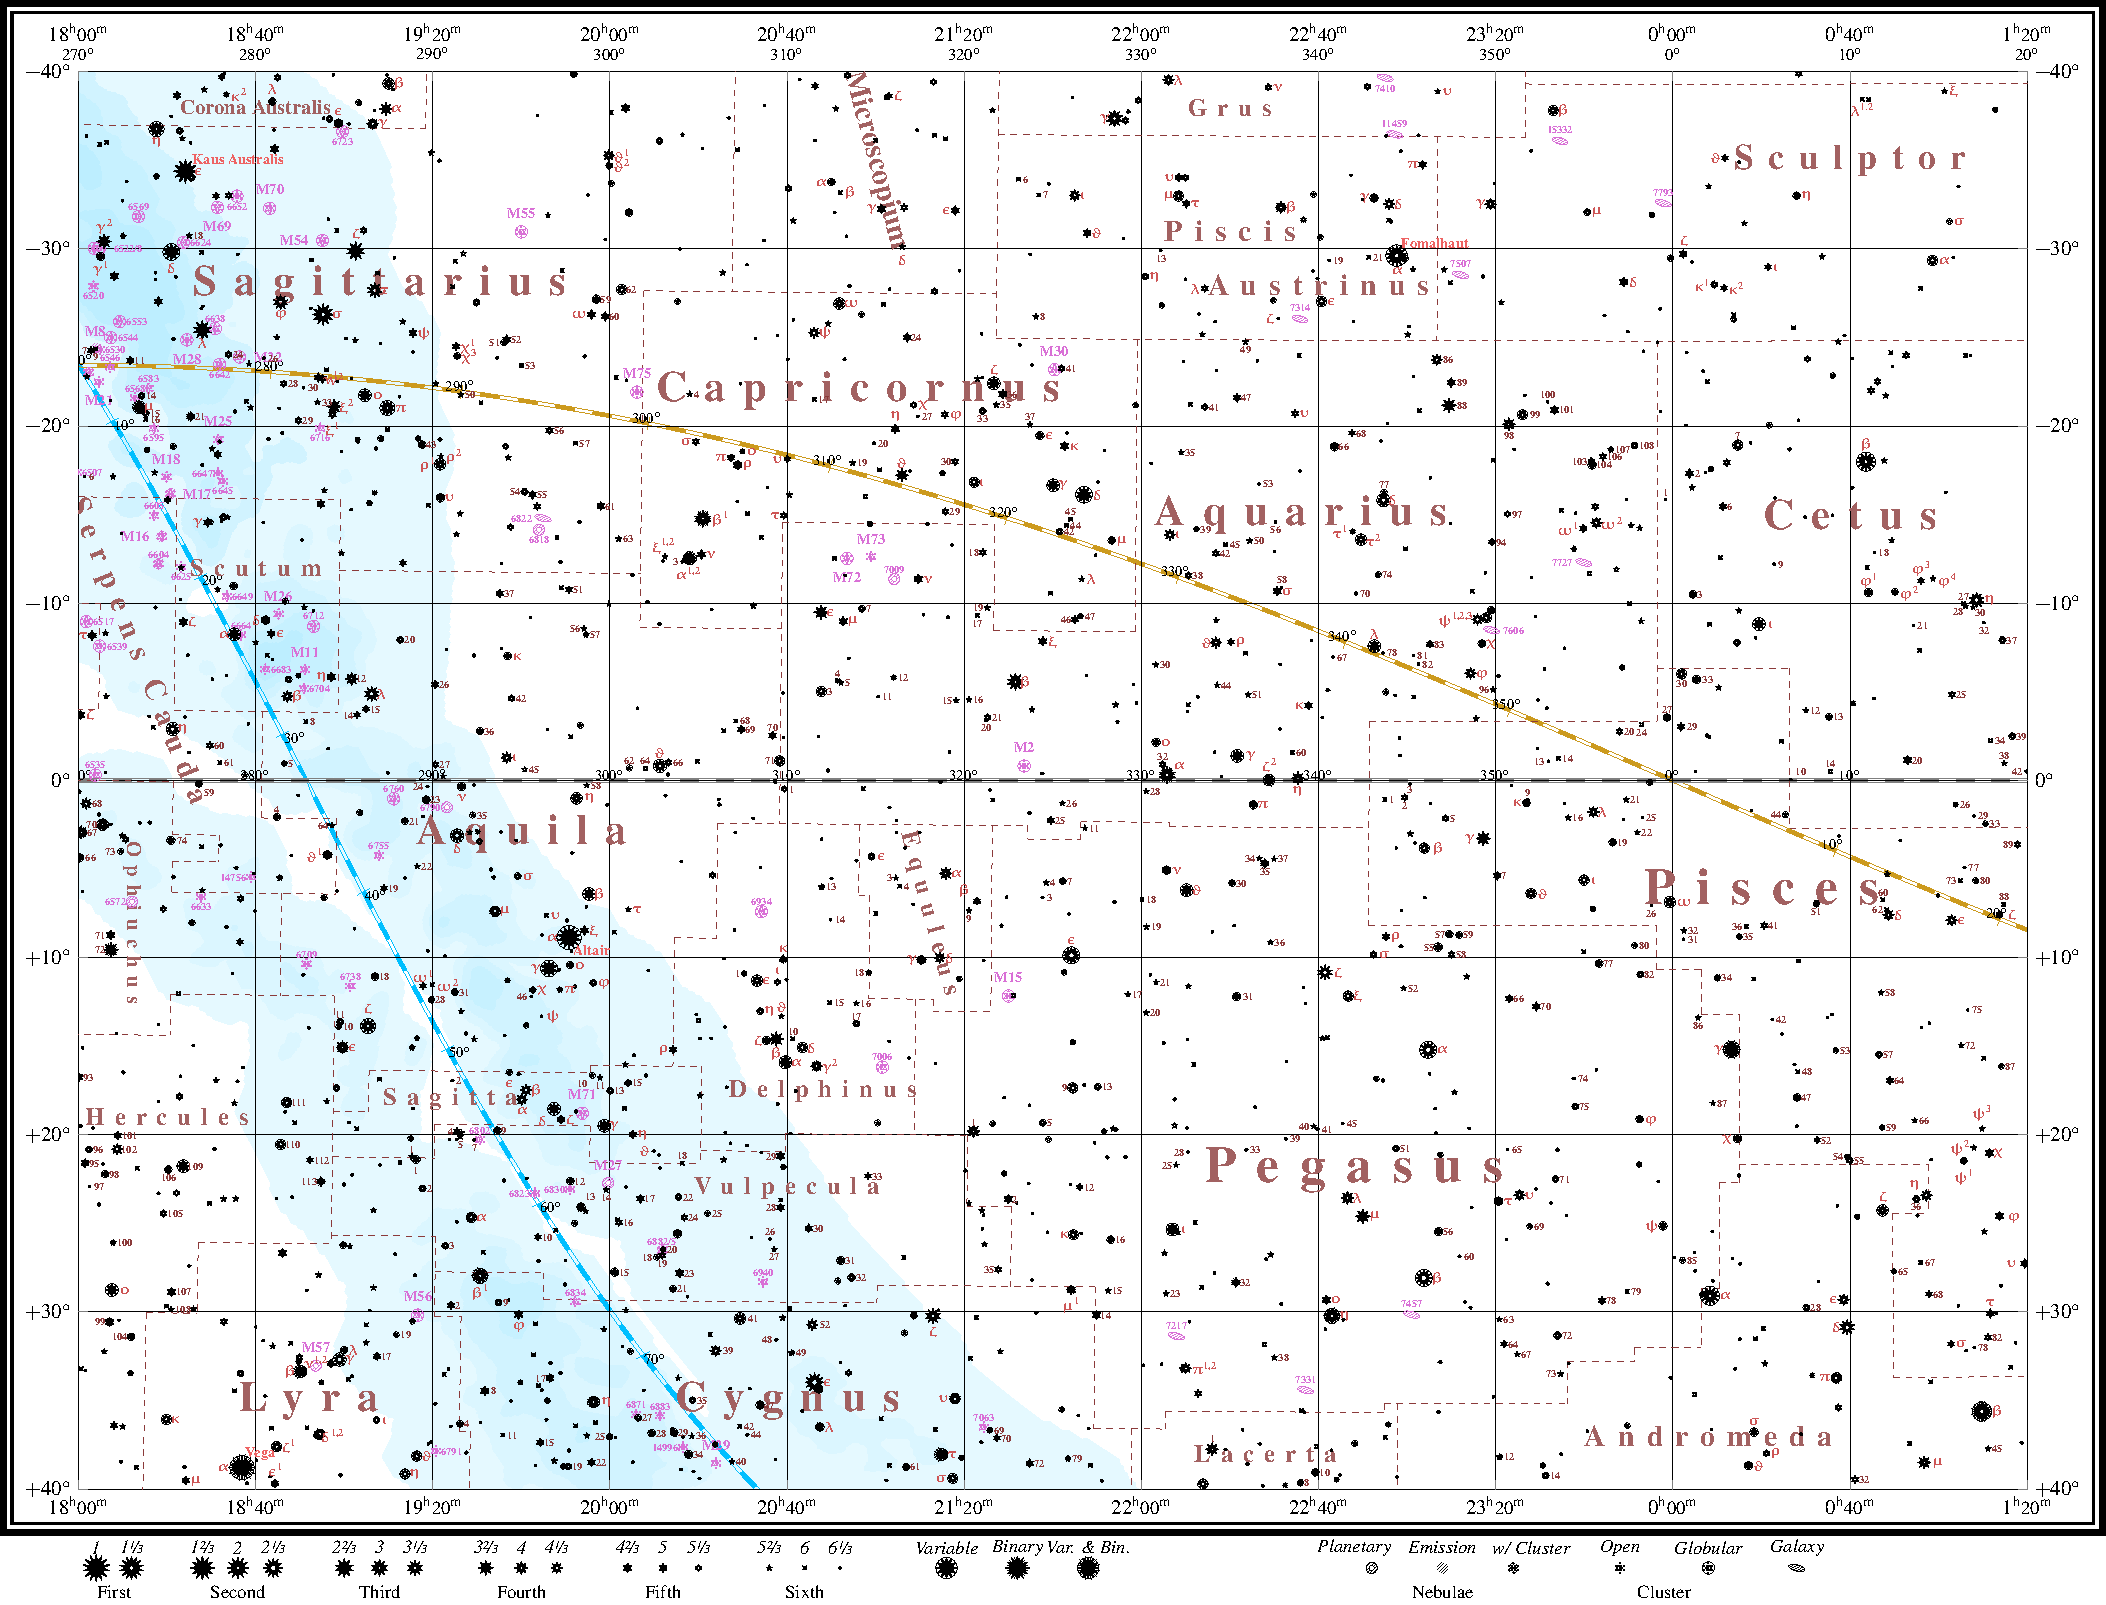
\includegraphics[height=0.963\textheight]{TabulaVI_S.pdf}\\[-0.985\textheight]\hfill\large~Tabula IV-S\hspace{25mm}
\clearpage
%
\noindent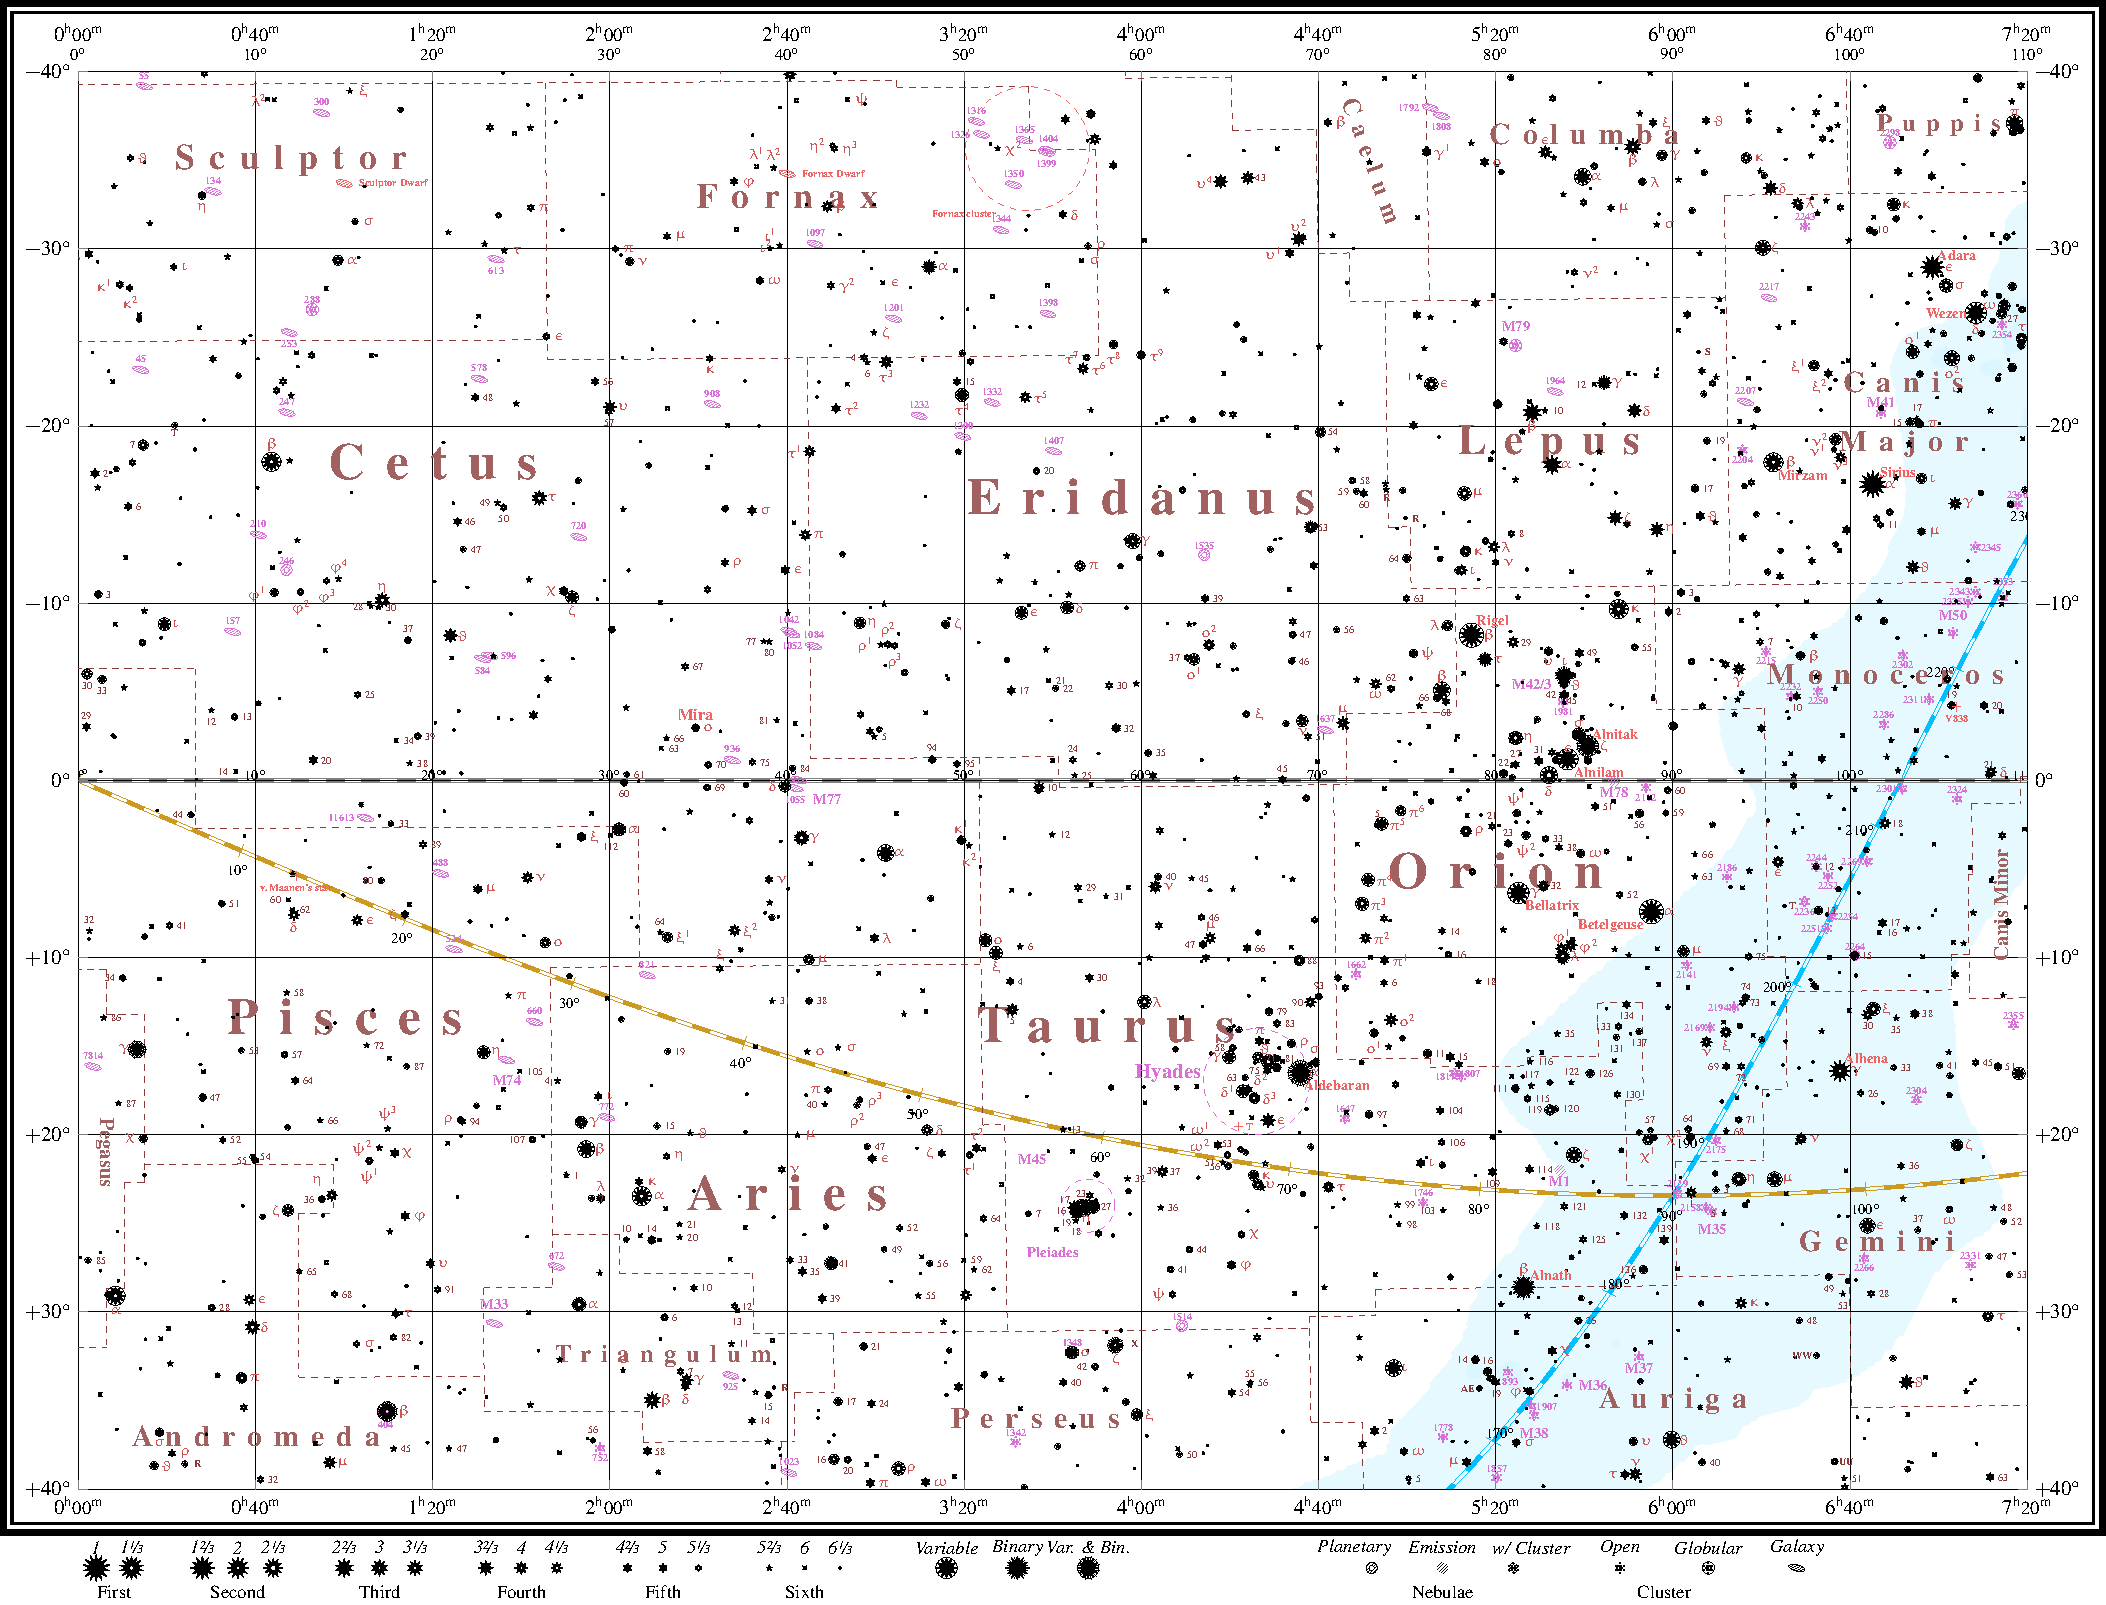
\includegraphics[height=0.963\textheight]{TabulaIII_S.pdf}\\[-0.985\textheight]\hfill\large~Tabula V-S\hspace{25mm}
\clearpage
%
\noindent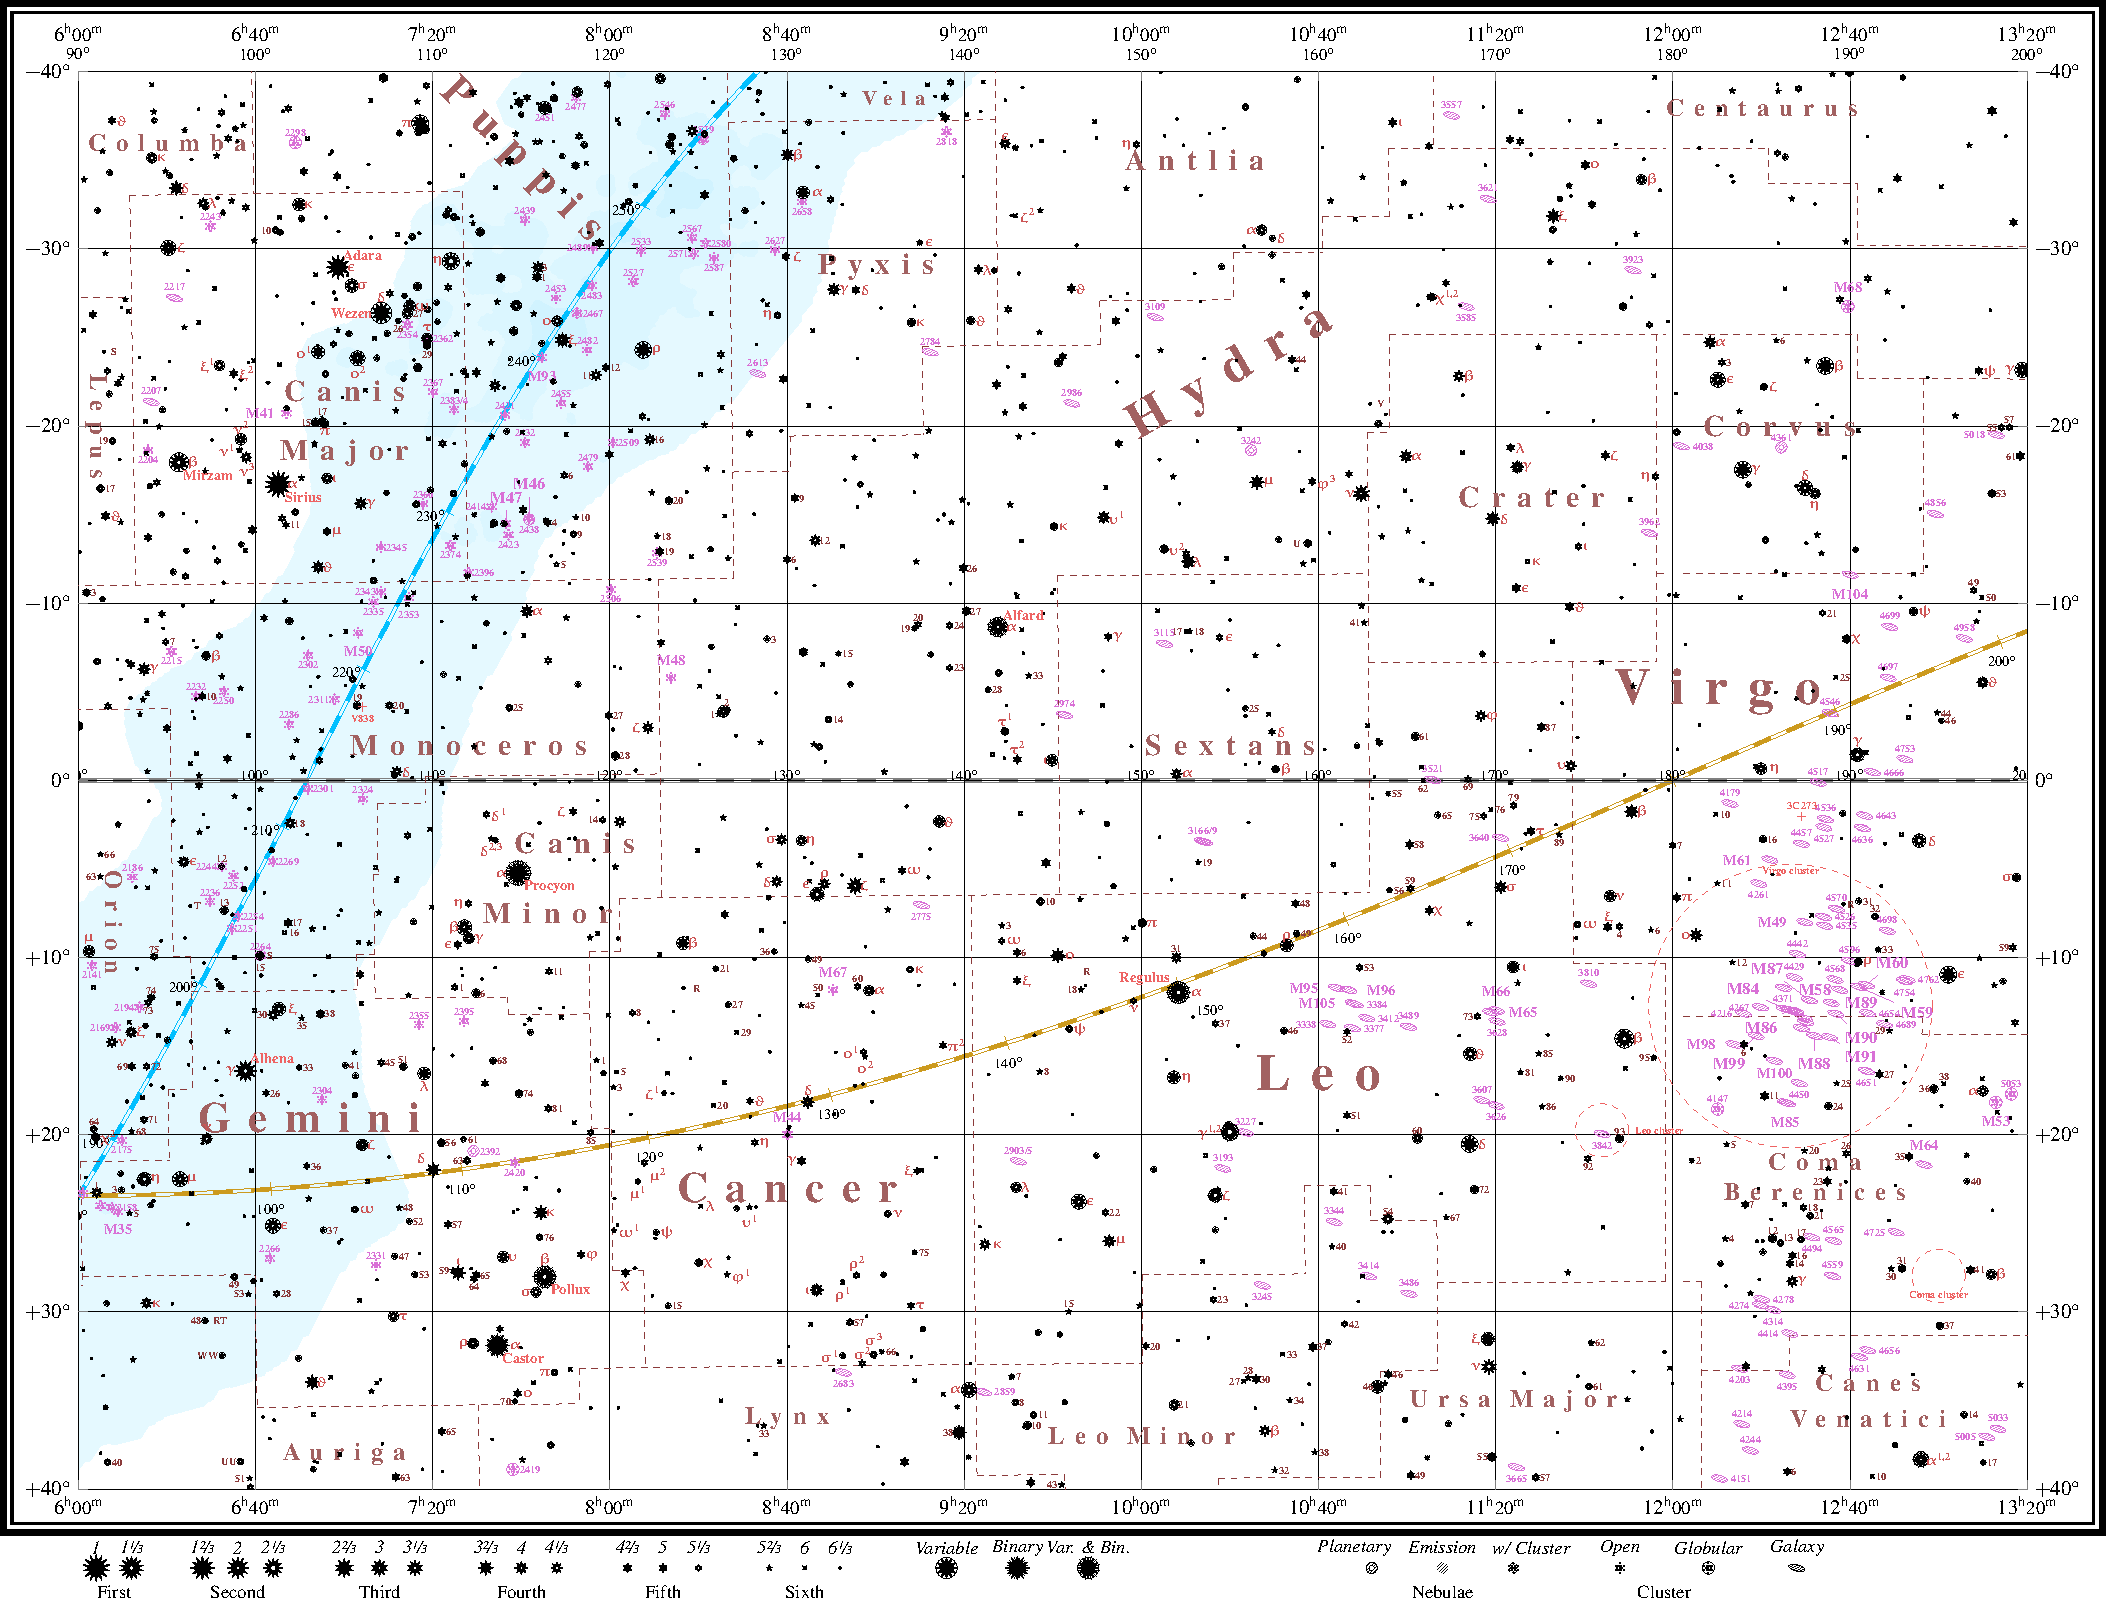
\includegraphics[height=0.963\textheight]{TabulaIV_S.pdf}\\[-0.985\textheight]\hfill\large~Tabula VI-S\hspace{25mm}
\clearpage
%
\noindent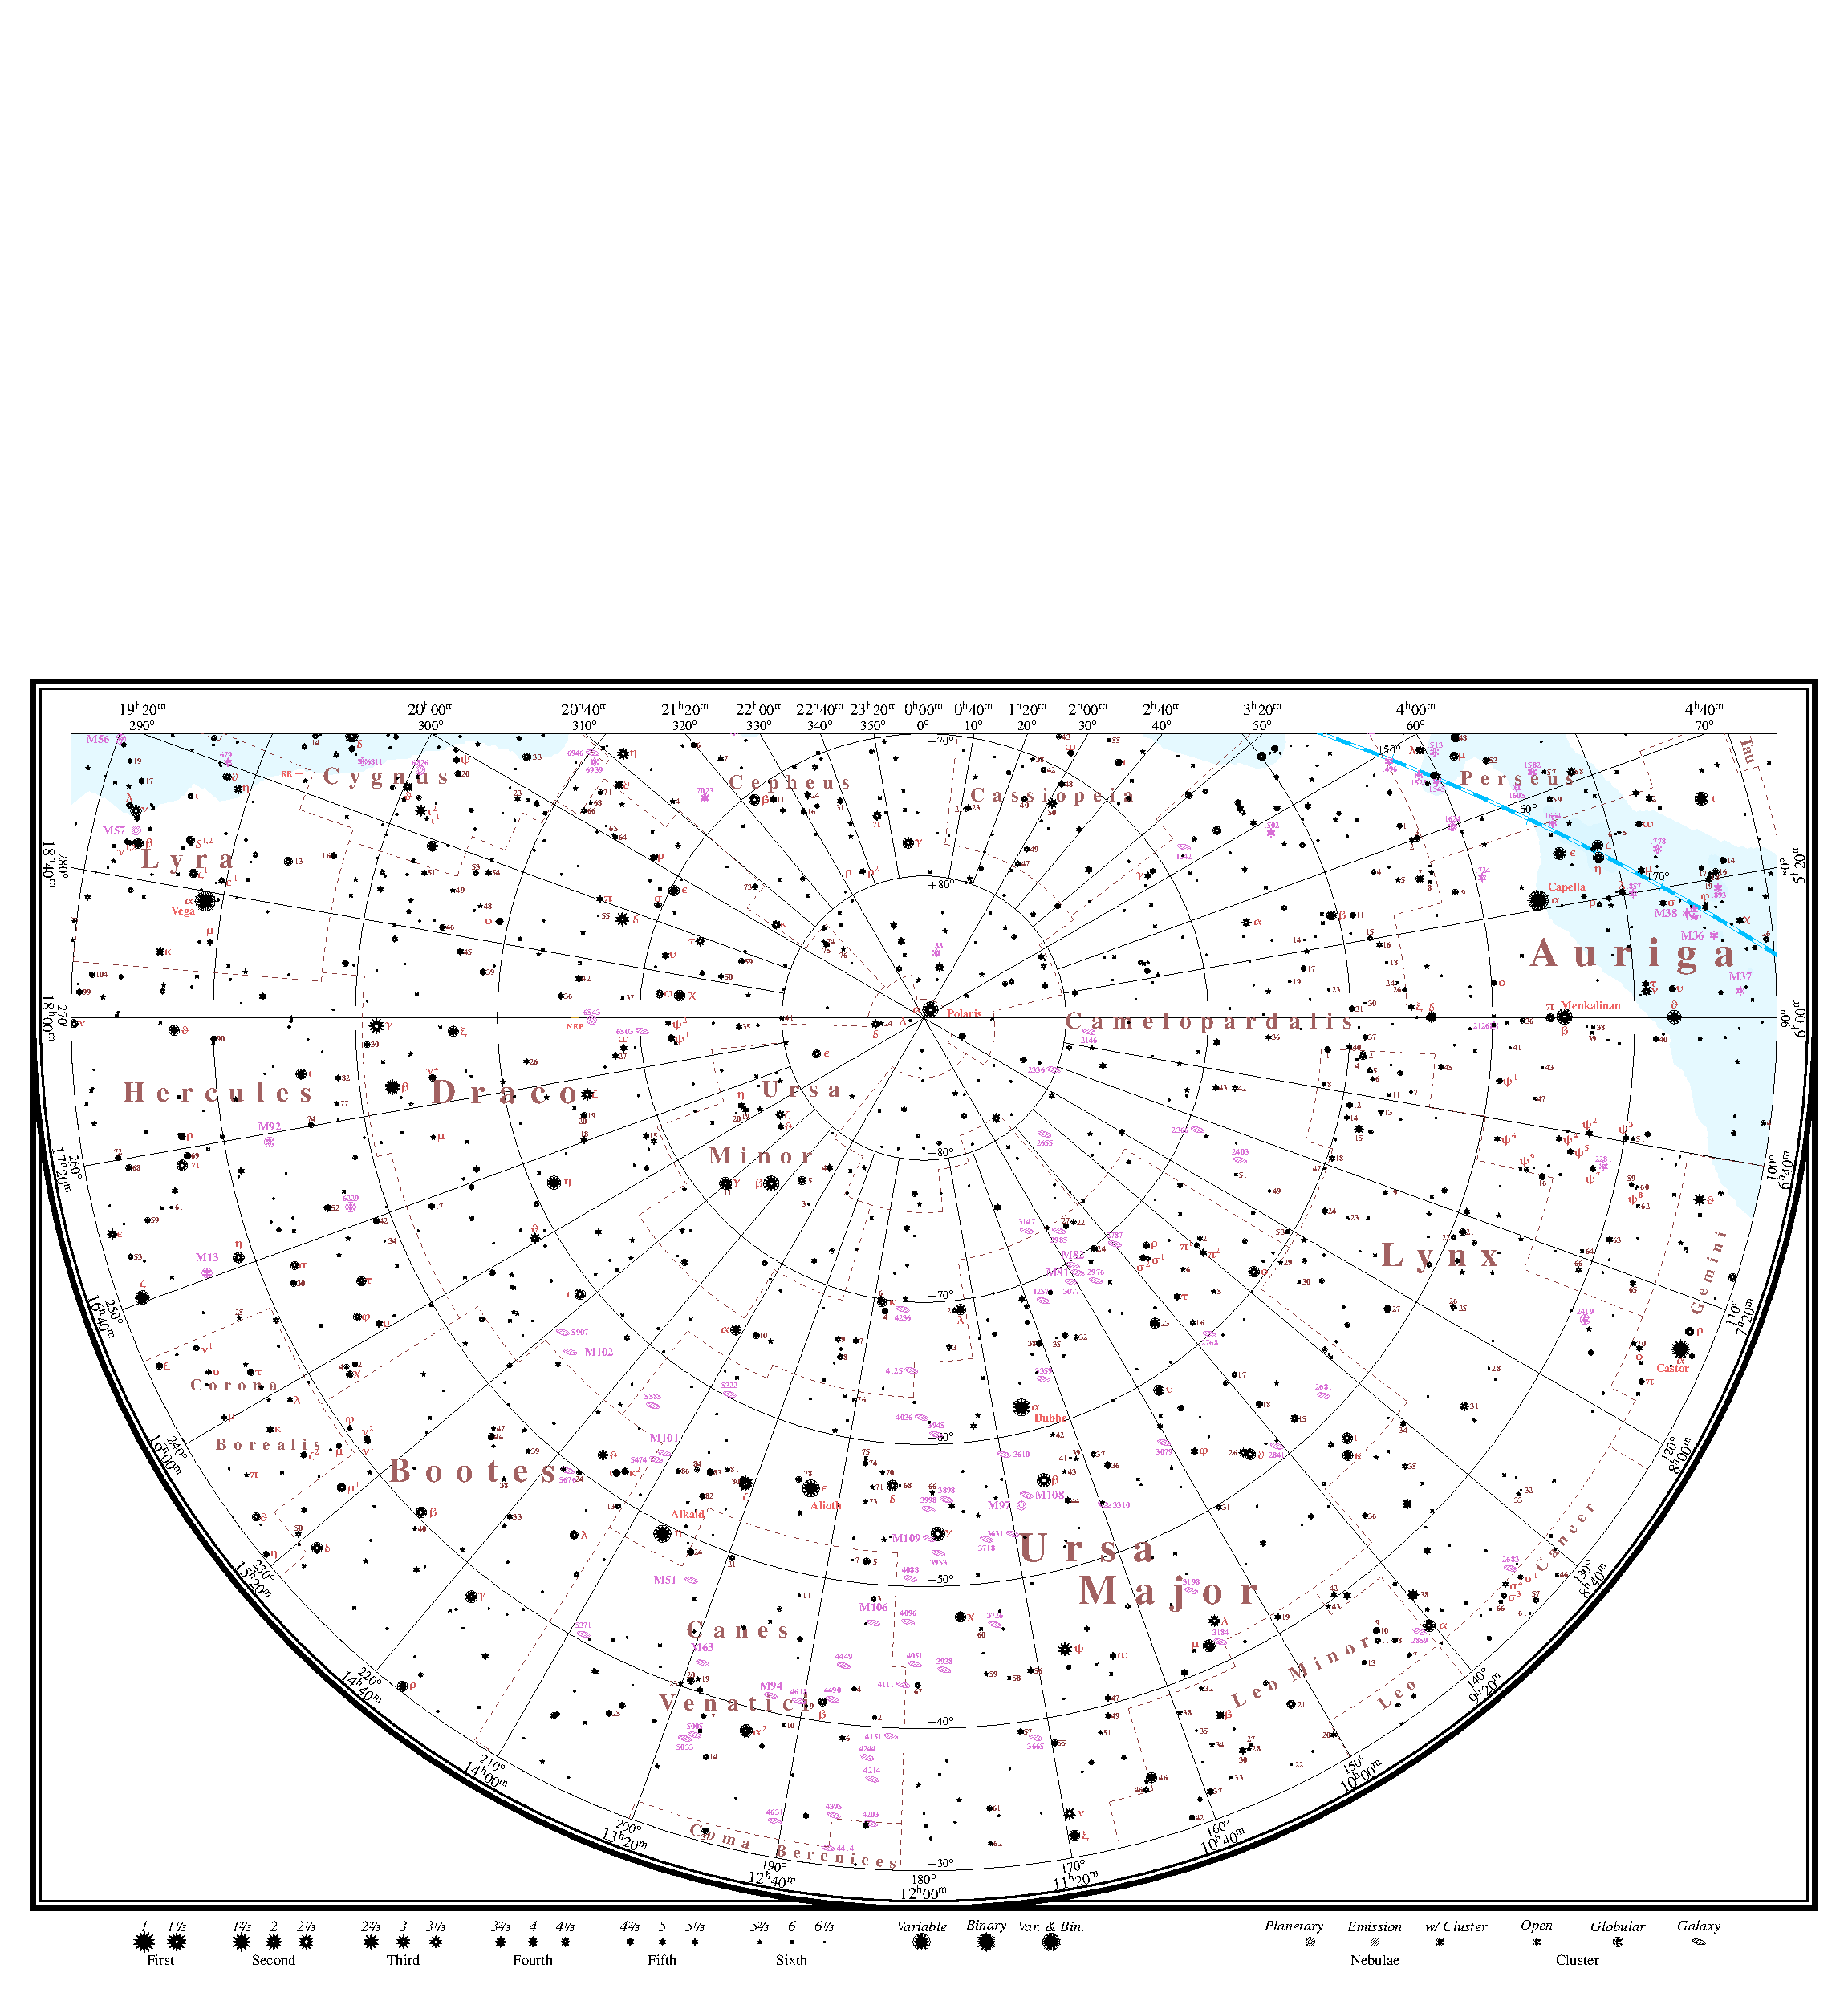
\includegraphics[height=\textheight,trim= 0.0cm 0.0cm 0.0cm 14.35cm,clip]{TabulaII.pdf}\\[-1.025\textheight]\hfill\large~Tabula VII-S\hspace{15mm}
\clearpage
%
\noindent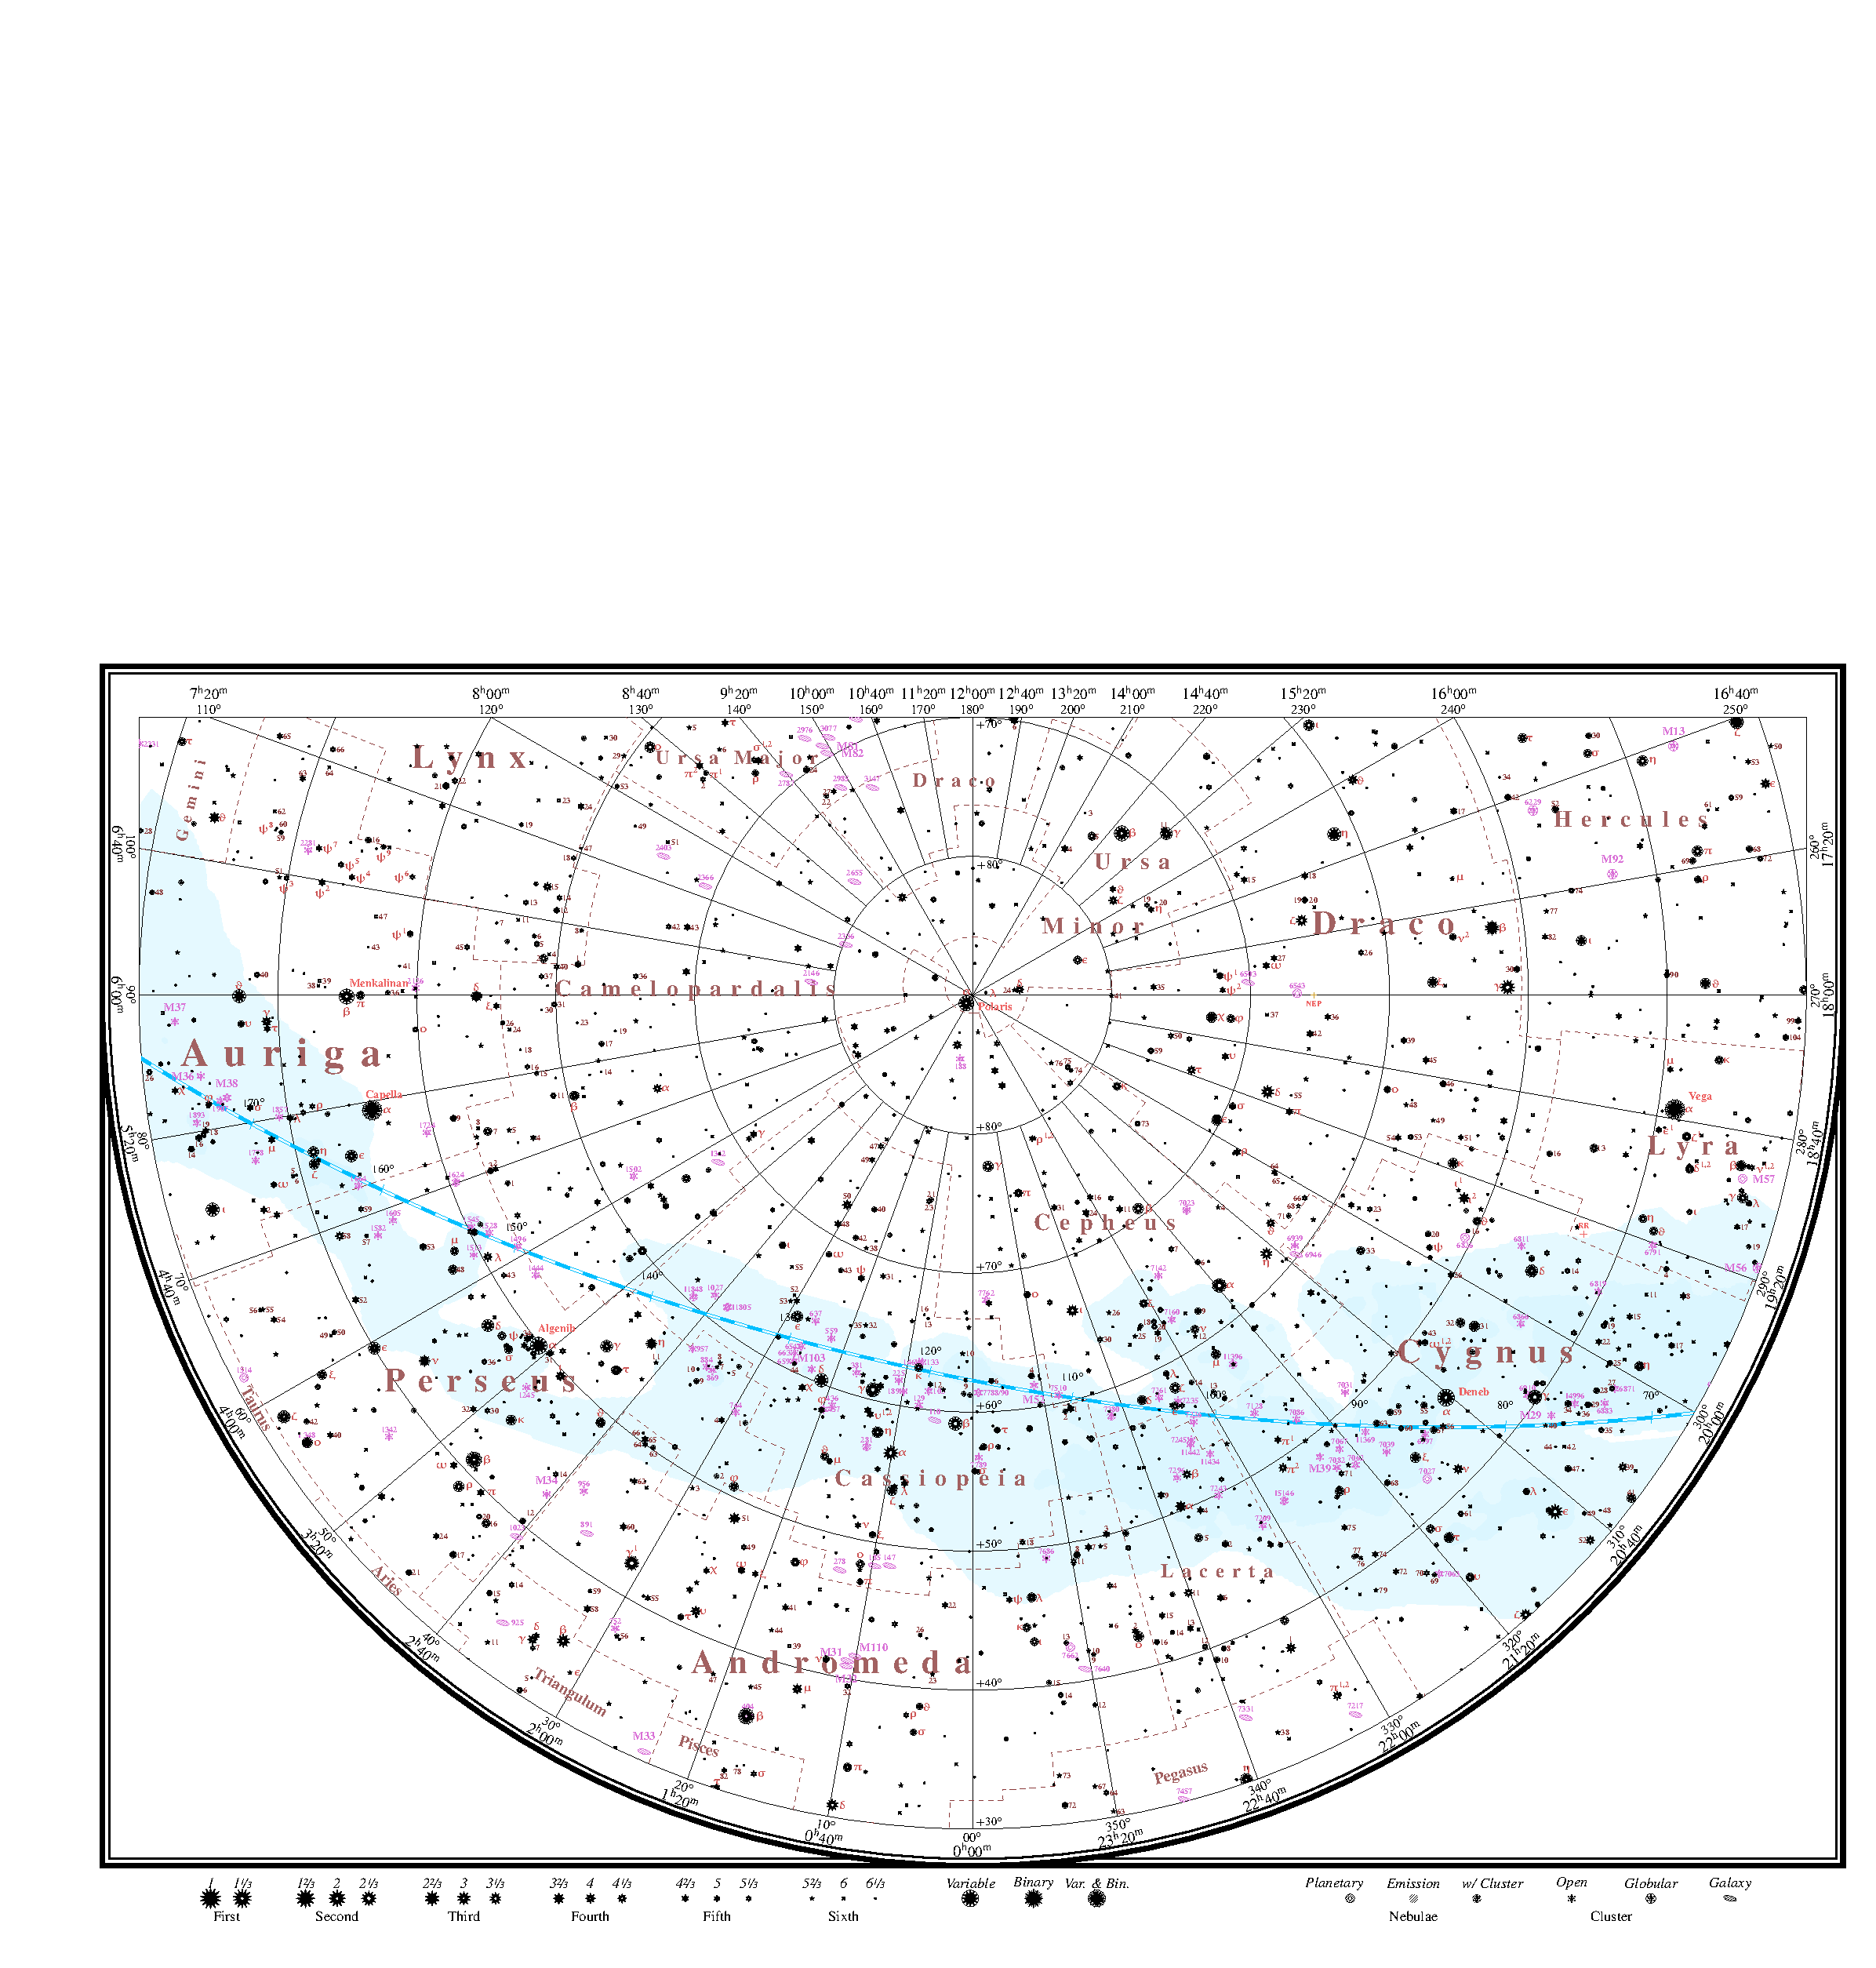
\includegraphics[height=\textheight,trim= 0.0cm 0.0cm 0.0cm 14.35cm,clip]{TabulaI.pdf}\\[-1.025\textheight]\hfill\large~Tabula VIII-S\hspace{7mm}
\clearpage
\end{center}

\end{document}
